\documentclass[12pt]{beamer}
\usetheme{Madrid}
\usepackage[utf8x]{inputenc}
\usepackage{ucs}
\usepackage{amsmath}
\usepackage{amsfonts}
\usepackage{amssymb}
\usepackage{graphicx}
\author{CHARPIGNON Thibault \\ GALLET Benoît \\ HERRMMAN Emmanuel \\ RETY Martin \\}
\title{GraphoScan}
\institute{ Université d'Orléans \\ \medskip \textit{Encadré par : EXBRAYAT Matthieu} }

\begin{document}

\begin{frame}
\titlepage
\end{frame}

\begin{frame}
\frametitle{Introduction}
\framesubtitle{Paléographie}
\begin{definition}
Science de l'étude des écritures manuscrites anciennes
\end{definition}
\begin{block}
\end{block}
\end{frame}

\begin{frame}
\frametitle{Plan}
\tableofcontents
\end{frame}

\section{Projet Originel}
\section{Travail Réalisé}
\section{Projet Final}
\section{Conclusion}

\begin{frame}
\Huge{\centerline{Projet Originel}}
\end{frame}

\begin{frame}
\frametitle{Projet Originel}
\framesubtitle{Travail Effectué}
\begin{itemize}
\item{C++ avec OpenGL, OpenCV et Matlab}
\item Structure :
\begin{figure}
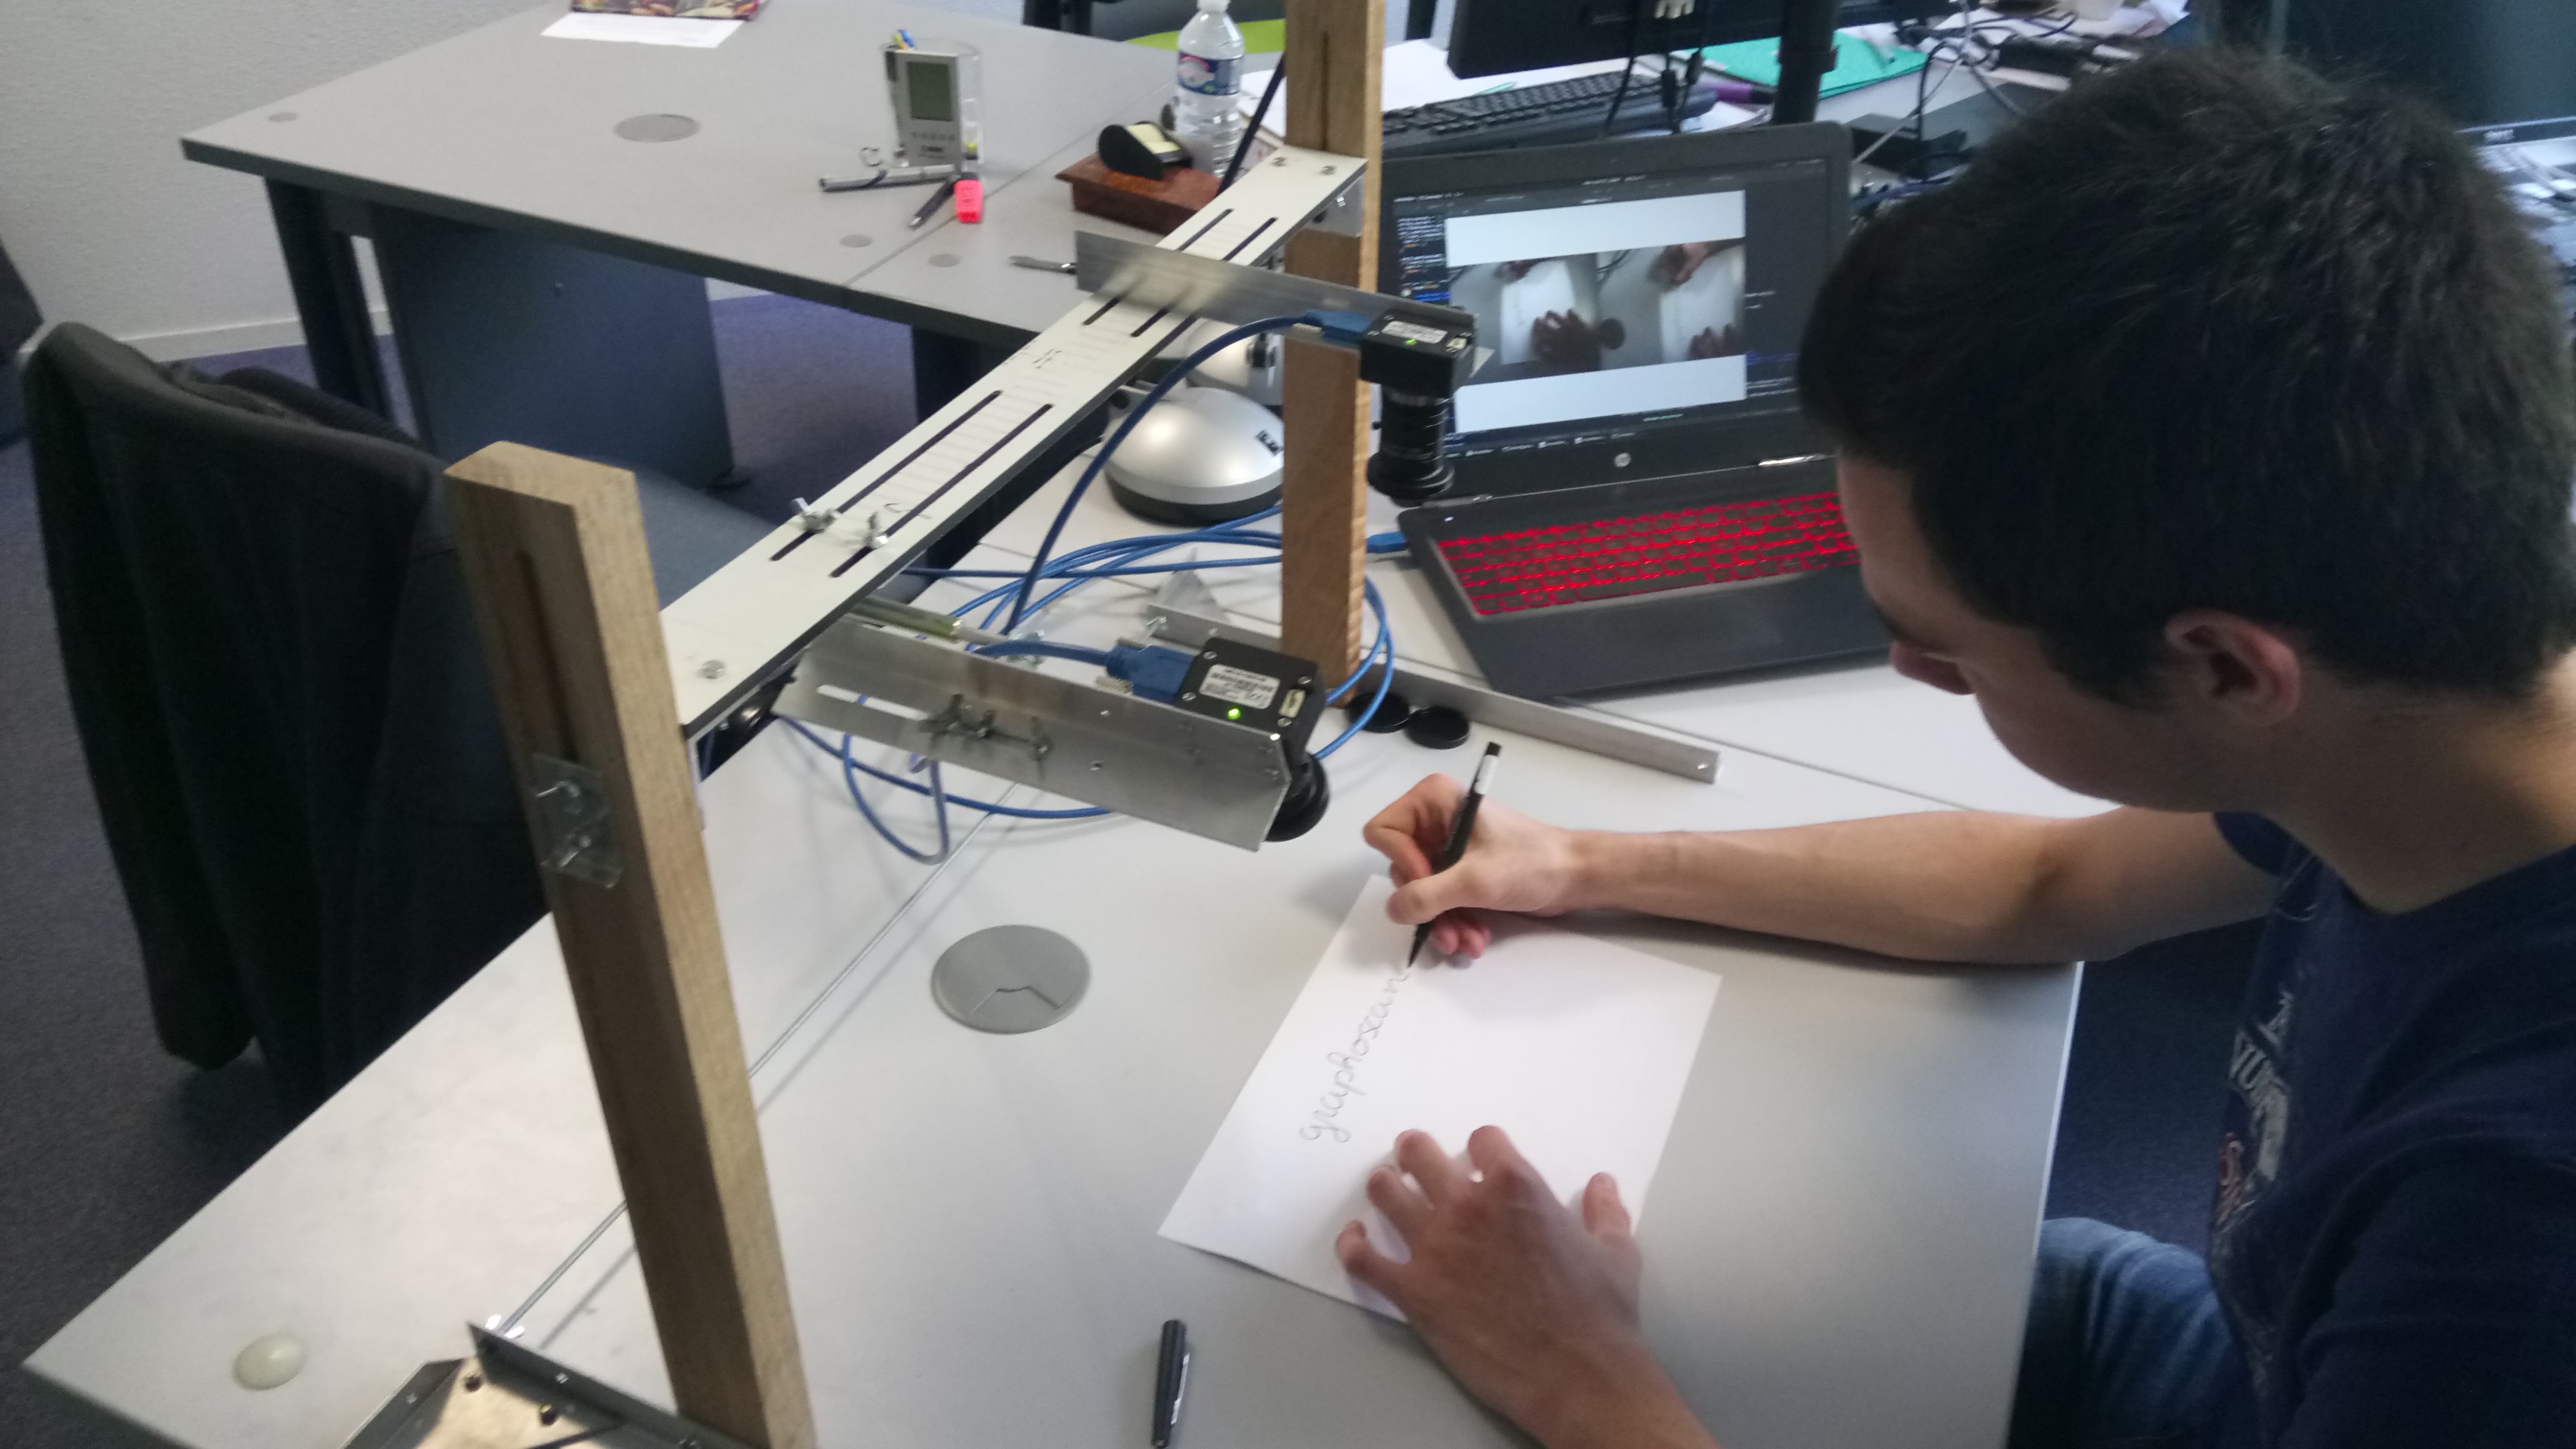
\includegraphics[width=0.5\textwidth]{../Rapport/Modules/Picture/Utilisation.png}
\end{figure}
\end{itemize}
\end{frame}

\begin{frame}
\frametitle{Projet Originel}
\framesubtitle{Travail Effectué}
\begin{enumerate}
\item Acquisition vidéo
\begin{itemize}
\item Calibrage des caméras
\item Acquisition en stéréo
\item Correction de la distorsion pour lisser l'image
\end{itemize}
\item Tracking
\begin{itemize}
\item Region d'interêt (ROI)
\item Histogramme de gradient orienté (HOG)
\end{itemize}
\item Reconstruction 3D
\begin{itemize}
\item Calcul des points 3D avec OpenCV
\item Reconstruction 3D avec OpenGL
\end{itemize}
\end{enumerate}
\end{frame}

\begin{frame}
\frametitle{Projet Originel}
\framesubtitle{Problèmes}
\begin{itemize}
\item Fréquence d'acquisition trop faible (8 images par seconde)
\item Eclairage du dispositif trop faible entrainant des zones d'ombres
\item Déplacement du support d'écriture impossible
\item Geste de relaxation de l'utilisateur non gérés
\item Code non nettoyé, non documenté et copié depuis internet
\end{itemize}
\end{frame}

\begin{frame}
\Huge{\centerline{Travail Réalisé}}
\end{frame}

\begin{frame}
\Huge{\centerline{Projet Final}}
\end{frame}

\begin{frame}
\frametitle{Projet Final}
\framesubtitle{Vidéo de présentation}
\begin{enumerate}
\item Choix des images
\item Sélection de la ROI
\item Application de l'agorithme de tracking
\item Affichage des résultats
\item Affichage de la reconstruction 3D
\end{enumerate}
\end{frame}

\begin{frame}
\frametitle{Projet Final}
\framesubtitle{Améliorations possibles}
\begin{itemize}
\item Droit d'auteur
\item Interface graphique
\item Amélioration du tracking
\begin{itemize}
\item Déplacement de la feuille
\item Mouvements parasites
\end{itemize}
\item Synchronisation native
\item Reconstruction 3D
\end{itemize}
\end{frame}

\begin{frame}
\frametitle{Conclusion}
\end{frame}

\end{document}